% numerics.tex      pdflatex ZhCvGo15
% Diffuse globally, compute locally: a cyclist tale
% Tingnan Zhang, Daniel I. Goldman and Predrag Cvitanovi\'c

%\subsection{Numerical results}
%                         was {Diffusion in the fundamental domain}
%\label{s-numerics}
\begin{table}[htbp]
	\centering
	\begin{tabular}{|r|r|r|l|l|}
		\hline
		${n_p}$ & \# cycles & $\zeta$(0,0) & $\lambda$ & D \\ 
		\hline\hline
		1      & 0      &   -    &   -  &   - \\
		2      & 24     & -0.31697 & 1.330 & 0.375\\
		3      & 64     & -0.54152 & 1.435 & 0.339\\
		4      & 168    & -0.09764 & 1.902 & 0.284\\
		5      & 516    &  0.02334 & 2.324 & 0.215\\
		6      & 1589   & -0.00481 & 1.975 & 0.133\\
		7      & 5700   & -0.01241 & 1.885 & 0.184\\
		8      & 20729  & -0.01006 & 1.785 & 0.247\\ \hline
	\end{tabular}
	\caption[Elementary cell cycle expansion results of diffusion 
	coefficient]{\label{TCELL1}
		Elementary cycle expansion results~\refeq{eq-diff-ec} computed
		Schreiber 1992 calculation\rf{CGS92} (and this paper) in the
		elementary cell.}
\end{table}

Elementary cycles and the corresponding cycle expansion calculation
results are listed in \reftab{TCELL1}. Although the diffusion
coefficient computed using elementary cycles up to $n_p = 8$ is close 
to the numerical experiment value $0.25$, the convergence is not
promising, as have pointed out in~\refref{CGS92, Morriss1994}.

\begin{table}[htbp]
	\centering
	\begin{tabular}{|r|r|r|l|l|}
		\hline
		$\period{p}$ & \# cycles & $\zeta$(0,0) & $\lambda$ & D \\ 
		\hline\hline
		1      & 5      & -0.2169759 & 1.39193 & 0.37795 \\
		2      & 10     & -0.0248233 & 1.74541 & 0.23118 \\
		3      & 33     & -0.0221962 & 1.72235 & 0.25257 \\
		4      & 108    & -0.0002192 & 1.74450 & 0.24165 \\
		5      & 373    &  0.0023463 & 1.76079 & 0.24468 \\
		6      & 1378   &  0.0096330 & 1.75610 & 0.24068 \\ 
		\hline\hline
		\multicolumn{3}{|l|}{numerical experiment}
		& 1.760   & 0.25
		\\ \hline
	\end{tabular}
	\caption[Fundamental domain cycle expansion results of diffusion 
	coefficient]{\label{TCELL2}
		Results for $w$=0.3. Calculation in the fundamental domain . 
		Gaspard 
		1992 note: ``My
		numerical estimate for the Lyapunov exponent when $w=0.3$ is
		$\lambda = 1.760 \pm 0.002$, which supports the result of this
		table.'' The numerical diffusion coefficient is calculated 
		using 
		Green-Kubol method. 
	}
\end{table}

We list the numerical results computed using the fundamental domain
orbits (Equation~\refeq{eq-fd-msd}) in \reftab{TCELL2}. Compared with
other methods, the symmetry-reduced cycle expansion method converges
the fastest, see \reftab{TCELL2} and \reffig{fig-results}A. Diffusion
coefficient computed from $\sim2\,000$ fundamental domain cycles of
topological length up to 6 converges to two significant digits, while
the elementary cell calculation needs over $\sim 10\,000$ cycles in
order to converge.

\begin{figure}
	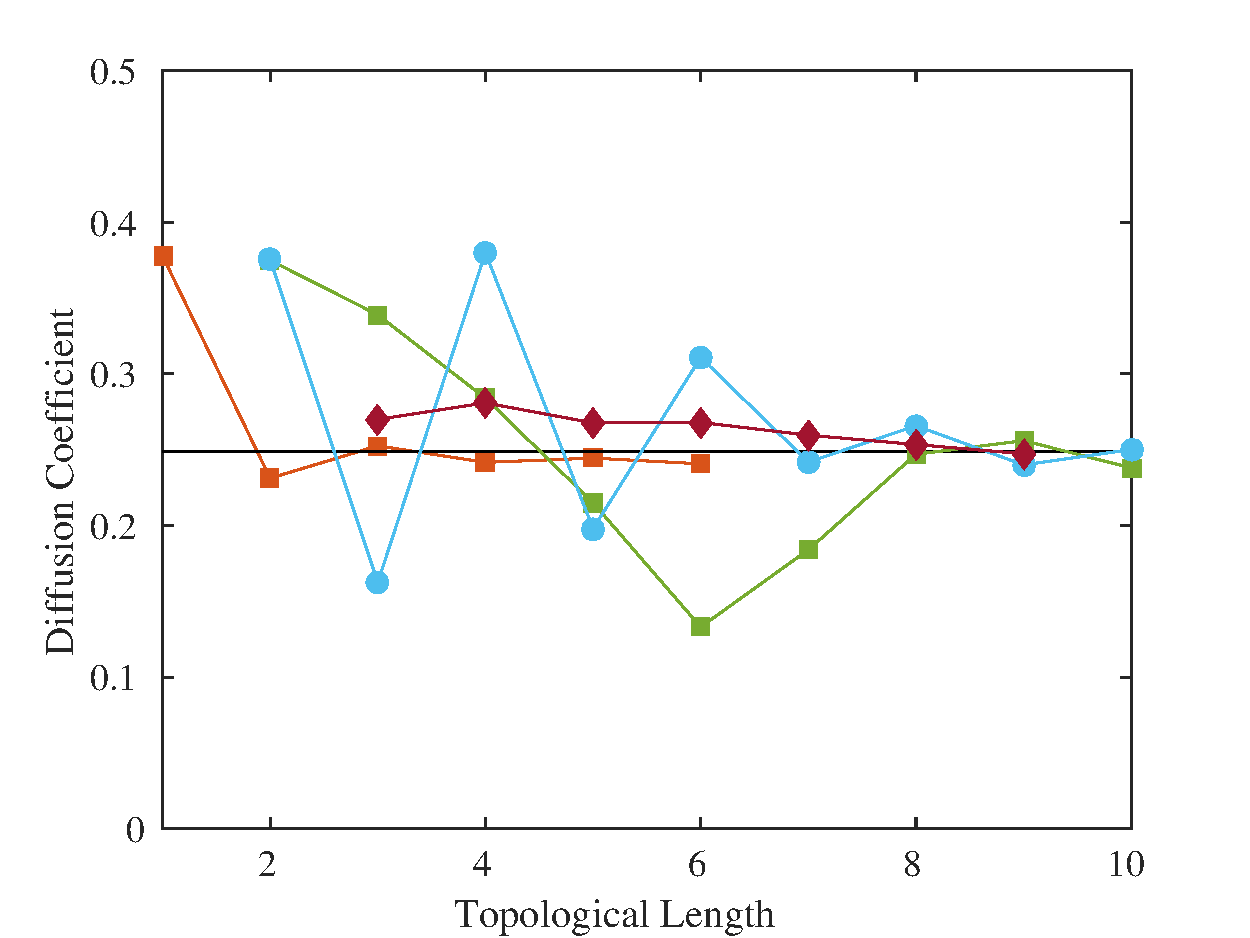
\includegraphics[width=0.5\textwidth]{diffuseCycleExpansionResults}
	\caption{\label{fig-convergence}The convergence of diffusion 
	coefficients  calculated using cycle		
		expansion in elementary cell (green squares), and fundamental 
		domain (orange squares). We also show the convergence of 
		``periodic orbit expansion'' method, with and  without Shanks 
		transformation (circles and diamonds) discussed in  
		\refref{Morriss1994}. Here $w = 0.3$.
		}
\end{figure}
\begin{figure}
	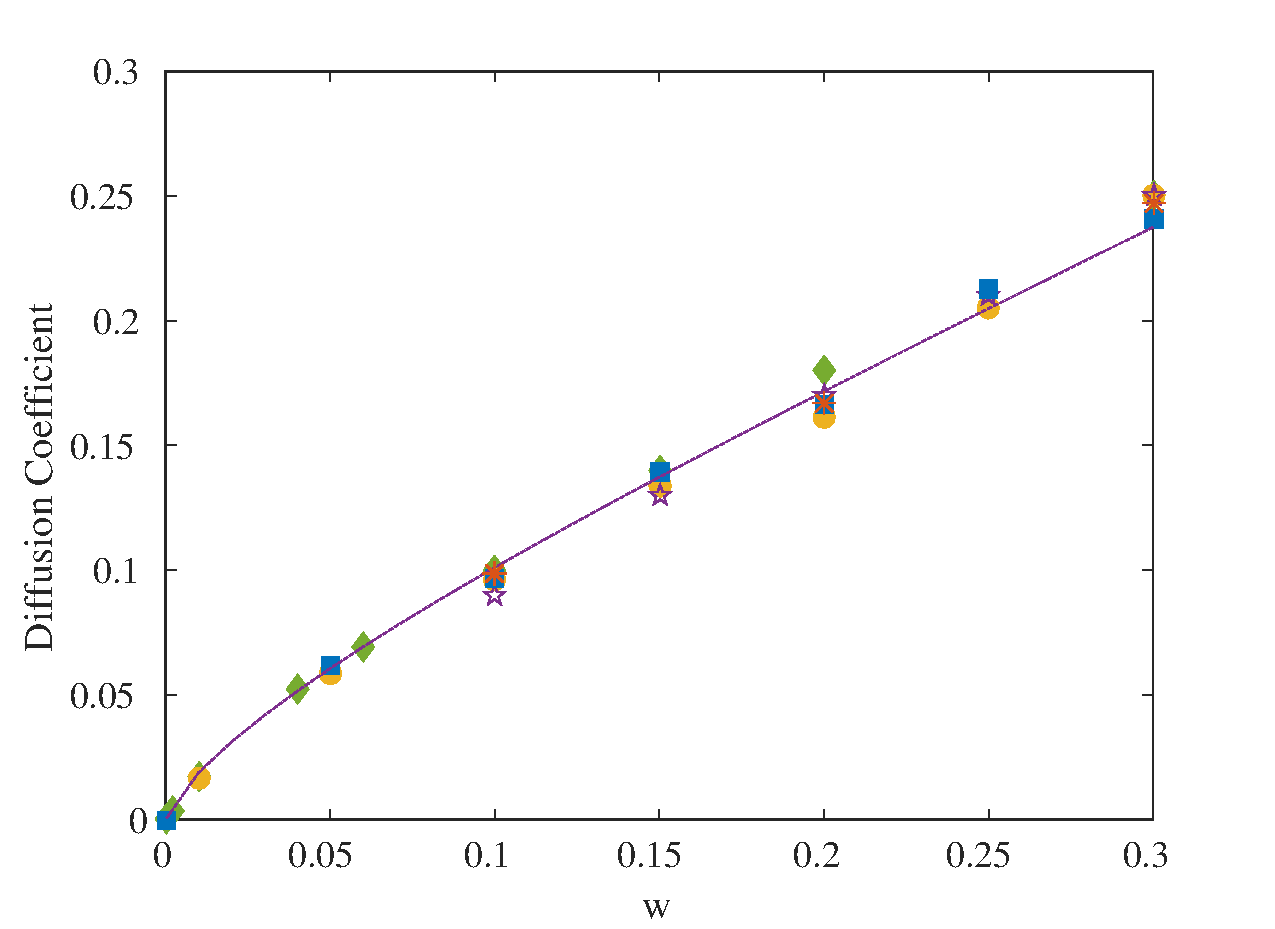
\includegraphics[width=0.5\textwidth]{diffuseDiffCoefPlot}
	\caption[Diffusion coefficients computed using cycle expansion 
	formulas]{\label{fig-results} 
		(A) The convergence of diffusion coefficients  calculated 
		using cycle
		expansion in elementary cell (green squares),  fundamental
		domain(orange squares). We  also show the convergence of 
		``periodic
		orbit expansion'' method, with and  without Shanks 
		transformation
		(circles and diamonds) discussed in  \refref{Morriss1994}. 
		Here $w =
		0.3$. (B) Diffusion coefficients as a function $w$.  Figure
		generated using data from various resources. Diamonds are 
		results
		from  Green-Kubo numerical experiments\rf{MacZwa83};
		stars\rf{BaEvCo93} and  circles\rf{GasBar95} are calculated 
		from
		escape rate; and triangles are  given by Hausdorff fractal 
		dimension
		calculation\rf{GasBar95}; dashed line  is a statistical
		approximation from\rf{AngMor12}.}
\end{figure}

We also compute the diffusion coefficient for $w = 0.05, 0.10, 0.15,
0.20, 0.25, 0.30$. The results are compared with previous numerical
experiments and a recent statistical estimation, see
\reffig{fig-results}. In Green-Kubo velocity auto-correlation method
the  diffusion coefficient can be extrapolated to the accurate
reference value $0.250$ (at $w/r=0.30$), using ensembles of
$10^6\sim10^7$ random trajectories that fly for an extensive period
($T > 20$)\rf{MacZwa83}. The number of bounces for each trajectory are
typically greater than $20$ (as compared to 6, the topological length
of longest periodic orbit we used). On the other hand, while
statistical approach yields a smooth analytical formula\rf{AngMor12},
the diffusion property in such systems is fundamentally never a 
smooth function of parameters\rf{Cristad06}. Unfortunately, for 
the 2D system we do not have enough numerical precision to monitor 
the fractal behavior of diffusion coefficient observed in 
\refref{Cristad06}. 

TODO

the 3 discrete and continuous average in the long time limit
